
Scalar active systems are those whose large-scale dynamics is well captured by a real (scalar) field, hereafter denoted $\rho$. 
As we have seen in chapter~\ref{chap_intro}, the field $\rho$ is usually referred to as the \emph{order parameter} of the theory.
While it can in general represent various quantities related to the dynamics, here it will be most of time given by the particle density.

% At equilibrium, the minimal continuous description of scalar systems with conserved order parameter is achieved via \emph{model B} (see~\cite{HohenbergRMP} for a comprehensive classification).
% Model B indeed describes a class of equilibrium systems whose dissipative dynamics is captured by a conserved field, such that $\intd{r} \, \phi(\bm r,t) = {\rm const}$, for all times $t$,  where hereafter the variables $\bm r$ and $t$ account for space and time, respectively, while $d$ denotes the number of spatial dimensions.
% As model B describes the universal large-scale features of many systems, it can be formulated based on relevant symmetries and conservation laws.
% Such a phenomenological approach can moreover be supplemented by direct coarse-graining from microscopic (particle-based) theories, which provide additional physical insights. 

% In these notes, we will apply both approaches---phenomenological and coarse-graining---to study the dynamics of scalar active systems.
% We begin with a bottom-up approach
% In \autoref{chapter: introduction}, we introduced the active Brownian particle (ABP). 
% By extending this model to a collection of interacting ABPs, we will employ coarse-graining techniques to obtain one of the paradigmatic examples of collective active matter, motility-induced phase separation (MIPS).
% Here we will review some of the essentials of equilibrium phase separation physics, what changes for methods that do not admit an equilibrium description, and discuss what is needed for this to be the case.
% We will then take a more phenomenological approach to derive the Active Model B (AMB) and the Non-Reciprocal Cahn-Hilliard (NRCH) model, and explore their rich out-of-equilibrium features.



\section{Interacting active Brownian particles}

\subsection{The microscopic model}

In \autoref{intro_ABM}, we have introduced a simple model of noninteracting active Brownian particles. 
Here, we consider the simplest extension of this model by assuming that we have isotropic particles that interact via volume exclusion. 
For simplicity, we restrict our analysis to two spatial dimensions, while most of what we present below also holds in $d=3$.

We thus have $N$ active particles defined by their positions $\bm r_i$ and self-propulsion orientations $\theta_i$, $i \in \{1, \dots N\}$.
As we have seen before, we can model their dynamics in terms of overdamped Langevin equations.
In two dimensions, these take the form
% The dynamics of each of these particles are described by an underdamped Langevin equation with an active velocity, as in \autoref{chapter: introduction}.
% Without interaction, it 
% %
% \begin{align}
%     \odv{\bm r_i}{t} = \bm v_{i,a}(t) + \sqrt{ 2 D_t } \bm \xi_i(t),
% \end{align}
% %
% where $\bm \xi_i(t)$ is white Gaussian noise, which obey
% %
% \begin{align}
%     \E{\xi_{k,i}(t)} &= 0, &
%     \E{\xi_{k,i}(t)\xi_{k',j}(t')} = \delta_{ij} \delta_{kk'} \delta(t - t').
% \end{align}
% %
% In two dimensions, the active velocity may be parametrized in terms of a single angle, $\bm v_a(t) = v_0 \hat {\bm e}(\theta(t))$, where 
% %
% \begin{align}
%     \hat {\bm e}(\theta) 
%     =
%     \begin{pmatrix}
%         \cos \theta \\ \sin \theta
%     \end{pmatrix}.
% \end{align}
%
%We focus on times much larger than the time scale of the rotational noise, $t\gg \tau_r = 1 / D_r$, so we may consider the rotational noise $\xi_i(t)$ to be white Gaussian noise as well.
%Including the interaction potential $U$, the full equations of motion for each particle becomes
%
\begin{subequations}
\label{eq_Langevin_int_ABPs}
\begin{align}
    \odv{\bm r_i}{t} & = v_0 \hat {\bm e}(\theta_i) - \frac{1}{\zeta} \nabla_{\bm r_i} U(\{\bm r_j\}) + \sqrt{ 2 D } \bm \xi_i, \\
    \odv{\theta_i}{t} & = \sqrt{ 2 D_r } \chi_i,
\end{align}
\end{subequations}
%
where $\zeta$ and $D$ correspond respectively to the friction and diffusivity, and are related by the relation $D = k_B T / \zeta$,
while $D_r$ denotes the rotational diffusivity of the self-propulsion direction, and the unit vector parametrizing the direction of self-propulsion takes the form
%
\begin{align}\label{unit vector}
    \hat {\bm e}(\theta) 
    =
    \begin{pmatrix}
        \cos \theta \\ \sin \theta
    \end{pmatrix}.
\end{align}
%
As before, the noises in~\eqref{eq_Langevin_int_ABPs} are Gaussian with zero mean, uncorrelated, and satisfy
\begin{equation*}
    \E{\xi_{k,i}(t)\xi_{k',j}(t')} = \delta_{kk'}\delta_{ij} \delta(t - t'), \qquad
    \E{\chi_{k}(t)\chi_{k'}(t')} = \delta_{kk'} \delta(t - t'). 
    %\qquad k,k' \in \{1,\ldots,N\}, \quad i,j \in \{1,2\}.
\end{equation*}
The interactions between the particles are modeled via a potential $U$, which we assume of the form
%
\begin{align*}
    U(\bm r_1, ..., \bm r_n) = \sum_{i \neq j} u(|\bm r_i - \bm r_j|).
\end{align*}
%
In the following, we also assume that $u$ is short-ranged, isotropic and repulsive: two particles only interact when they get in contact, while the amplitude and direction of the resulting force only depend on the vector joining their centers of mass.
The simplest choice satisfying these criteria is the hard-core potential 
\begin{equation*}
    u_{\rm HC}(r) = \begin{cases} +\infty & {\rm if}\; r < d_0\\
        0 & {\rm otherwise} \end{cases} ,
 \end{equation*}
with $d_0$ giving the particle diameter, 
that prevents any overlap between the particles.  
In practice --i.e. for simulations-- the hard core potential is often approximated via the Weeks-Chandler-Andersen potential (or truncated Lehnnard-Jones potential):
\begin{equation*}
    u_{\rm WCA}(r) = \begin{cases} 4\epsilon\left[ \left(\frac{d_0}{r}\right)^{12} - \left(\frac{d_0}{r}\right)^{6} \right] + \epsilon & {\rm if}\; r < 2^{1/6} d_0\\
        0 & {\rm otherwise} \end{cases} .
 \end{equation*}
Alternatively, one can also allow finite overlaps between particles by using a softer repulsion potential.
A common choice is the harmonic repulsion:
\begin{equation*}
    u_{\rm soft}(r) = \begin{cases} \tfrac{\epsilon}{2}(1 - r/d_0)^2 & {\rm if}\; r < d_0\\
        0 & {\rm otherwise} \end{cases} .
 \end{equation*}
 All the aspects that we describe below are qualitatively independent of the details of the interaction potential, 
 so that we do not make any specific choice in what follows. 

\begin{figure}[!t]
    \centering
    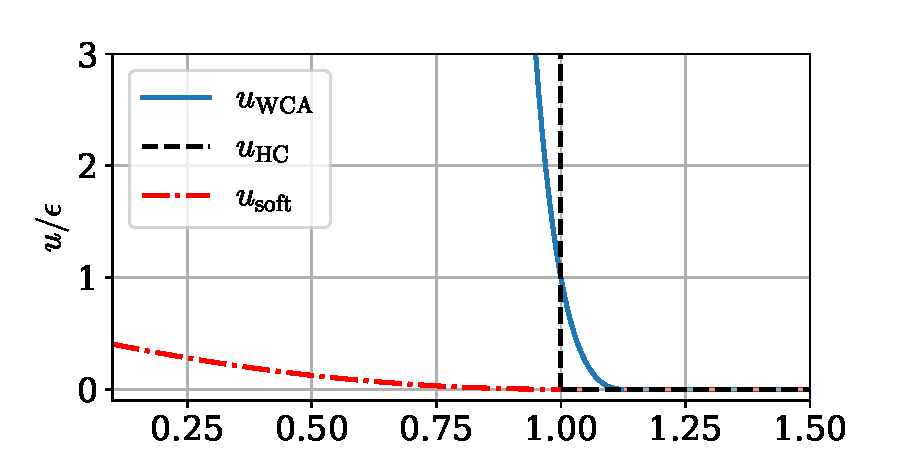
\includegraphics[width=.4\textwidth]{chapters/Figures/scalar/pot.pdf}
    \caption{Illustration of the possible choices for the potential $u$. A hard repulsion corresponds to $\lim_{r\to0} u(r) = +\infty$, such that the particles can never fully overlap. On the other hand, for the soft repulsion the maximum value of the potential is finite, such that overlaps are always possible.}
    \label{fig: hard soft}
\end{figure}

\subsection{Numerical simulations}

Rescaling space respectively with the particle diameter $d_0$ and time with the typical rotational diffusion timescale $\tau_r = 1/D_r$, Eqs.~\eqref{eq_Langevin_int_ABPs} read in dimensionless coordinates
\begin{subequations}
\label{eq_Langevin_int_ABPs_ND}
\begin{align}
    \odv{\bm r_i}{t} & = {\rm Pe} \, \hat {\bm e}(\theta_i) - \frac{\epsilon\tau_r}{\zeta d_0^2} \nabla_{\bm r_i} U(\{\bm r_j\}) + \sqrt{ \frac{2 D\tau_r}{d_0^2} } \bm \xi_i, \\
    \odv{\theta_i}{t} & = \sqrt{ 2 } \chi_i,
\end{align}
\end{subequations}
where we have defined $\epsilon$ as the unit scale of energies, while ${\rm Pe} = v_0\tau_r / d_0$ is usually referred to as the \textit{Péclet number}.

\textit{
{\bf Homework:}
From the relation $\int_{-\infty}^{+\infty}\dd t \,  \delta(t) = 1$, show that the physical unit of $\delta(t)$ corresponds to the inverse of a time. 
Use this result to deduce how the noises in Eqs.~\eqref{eq_Langevin_int_ABPs} rescale in dimensionless coordinates, and recover Eqs.~\eqref{eq_Langevin_int_ABPs_ND}. 
}

In dimensionless coordinates, the strength of activity, given by ${\rm Pe}$, is therefore set by the ratio of the persistence length of the active motion and the interaction range.
Simulating Eqs.~\eqref{eq_Langevin_int_ABPs_ND} in the low activity regime (i.e., either at low $v_0$ and/or low $\tau_r$), 
the dynamics qualitatively corresponds to that of an equilibrium gas of repelling particles.
On the other hand, when activity is increased sufficiently \autoref{fig: MIPS} shows that the particles spontaneously self-organize into a dense macroscopic domain coexisting with a surrounding dilute gas.
The densities of the dilute and dense phases are largely insensitive to variations of the mean particle density, which only set their relative volume fractions.
This phenomenology is thus similar to that of phase separation at equilibrium.
Here, however, there is no explicit attractive interactions between the particles, and the cluster formation finds its origin in the interplay of activity and crowding effects.
This collective behavior is known as \textit{motility-induced phase separation} (MIPS), and we will spend the following sections to explain its emergence. 
For detailed a review on MIPS that goes beyond the contents of this chapter, we recommend Ref.~\cite{}.

\begin{figure}[!t]
    \centering
    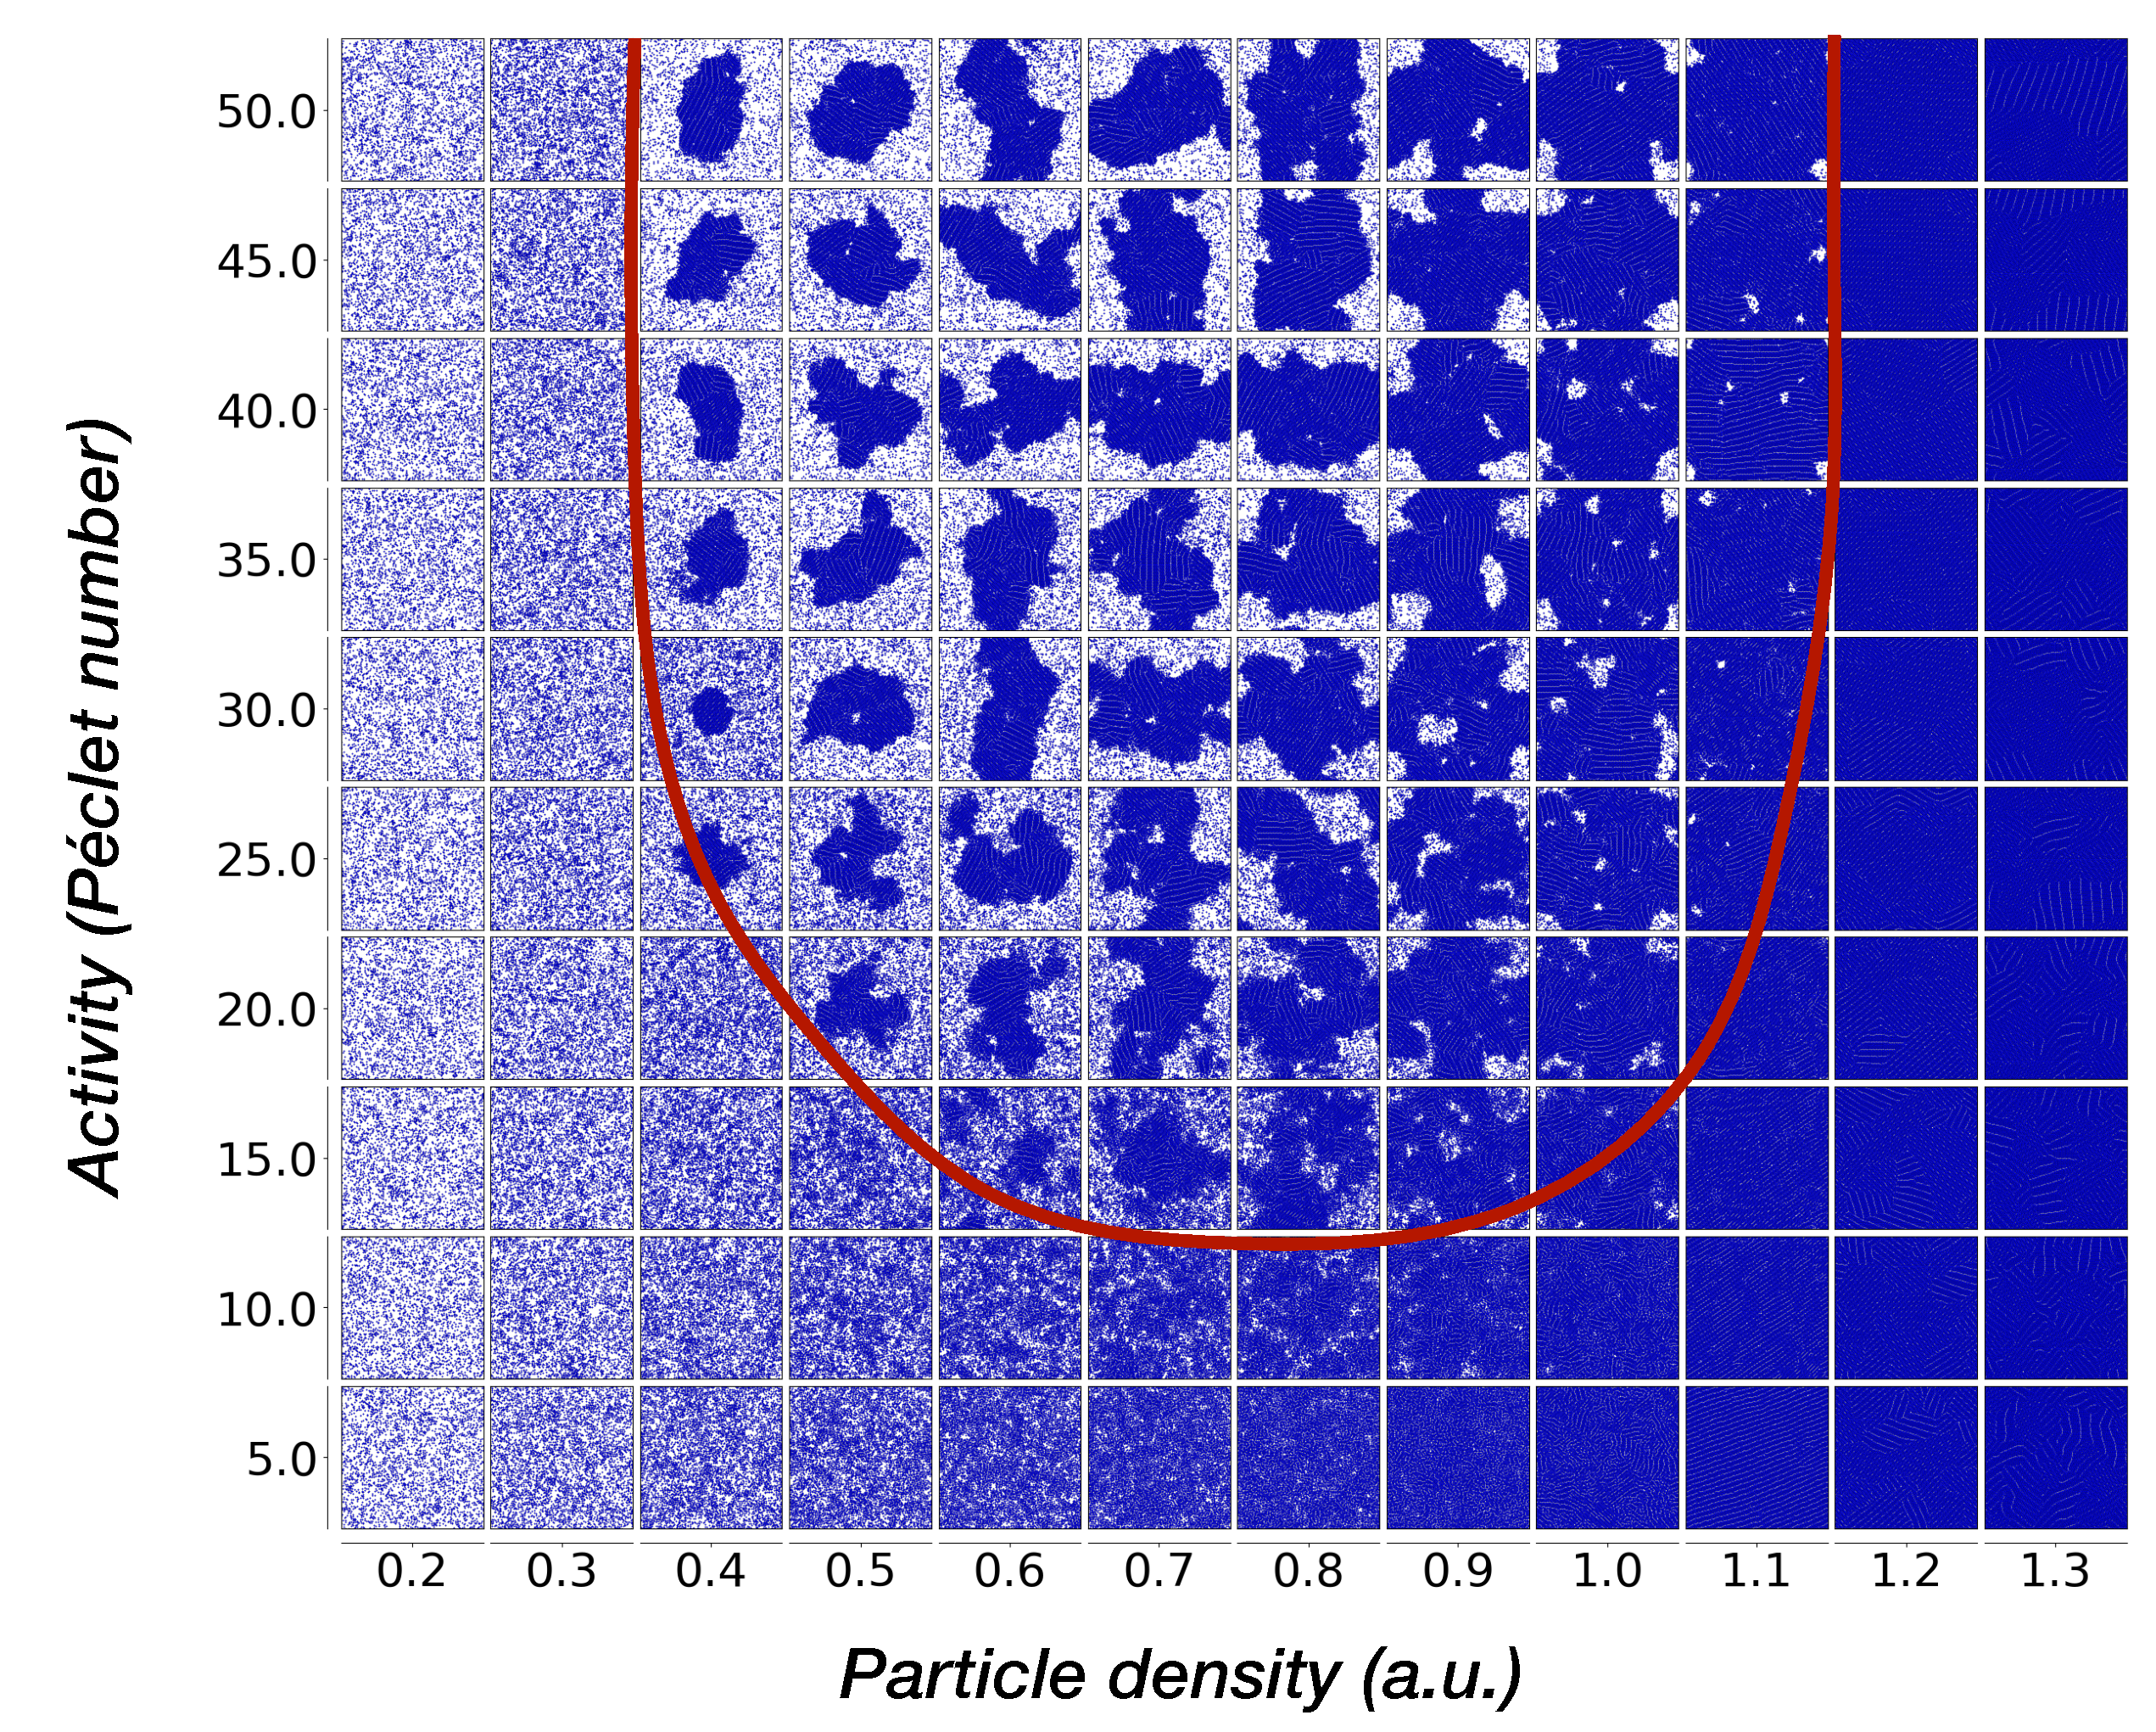
\includegraphics[width=.6\textwidth]{chapters/Figures/scalar/Fig_MIPS_PD.pdf}
    \caption{Phase diagram of the active Brownian particle model in the particle density - activity plane.
    Each panel shows a representative snapshot of the steady state configuration of the system.
    At large enough activity, the system undergoes a clustering instability, resulting in phase separated configurations where a dilute and a dense phase coexist.
    The red line serves as a guide for the eye to separate homogeneous and phase-separated configurations.
    \textit{Figure credits: Theo Spornhauer, University of Göttingen.}}
    \label{fig: MIPS}
\end{figure}

\subsection{The Mean field approach: a simple argument}

As the phenomenology of MIPS is qualitatively similar to that of equilibrium phase separation, we believe that it can be understood, as in the latter case, by an effective theory written in terms of the relevant field variable, which is here the particle density.
%As MIPS results from a many-body dynamics, it'll be better understood from a field theoretical description of the microscopic dynamics~\eqref{eq_Langevin_int_ABPs} expressed in terms of the relevant variables.
To achieve this, the usual procedure consist in writing the statistical description of the microscopic dynamics~\eqref{eq_Langevin_int_ABPs} in terms of the $N$-body particle distribution distribution,
%
\begin{align} \label{eq_PN}
    \calP_N(\{\bm x_i, \phi_i\}, t) = \E{ \prod_i \delta(\bm r_i(t) - \bm x_i)\delta(\theta_i(t) - \phi_i) },
\end{align}
%
whose evolution is ruled by the Fokker-Planck equation.
The particle density $\rho$ is then obtained from the single-body distribution $\calP(\bm x,\phi,t) = N\int\prod_{j=2}^N [\dd\bm x_j \dd\phi_j]\calP_N(\{\bm x,\phi,\bm x_2,\phi_2,\ldots,\bm x_N,\phi_N\},t)$ as
$\rho(\bm x,t) = \int\dd\phi \calP(\bm x,\phi,t)$.

If the particles are non-interacting, the probability distribution~\eqref{eq_PN} simply factors into $N$ independent single-body distributions. 
On the other hand, interactions introduce non-trivial correlations which prevent such factorization.
In this case the effective equation for the single-body distribution is a function of the two-body distribution, which itself depends on the three-body distribution, and so on. 
Obtaining the effective theory for $\calP(\bm x,\phi,t)$ thus requires to solve the so-called Bogoliubov-Born-Green-Kirkwood-Yvon (BBGKY) hierarchy.
It is in general impossible to do it exactly, so that achieving analytical progress requires to use a number of approximations.
While for those interested we present a derivation of the effective dynamics for $\calP(\bm x,\phi,t)$ in~\autoref{appendxi: BBKGY}, here we will instead focus on the describing the effective effect of the coupling between the particle self-propulsion and their repelling interactions by means of a mean field approximation.

Consider an isolated particle moving freely.
Its instantaneous self-propulsion speed is then given by $v_0$. 
If, on the other hand, our tagged particle enters a region of high density, it will begin to collide with other particles, and the main result of these collisions will be an effective self-propulsion speed $< v_0$.
To use a familiar analogy, imagine yourself running in an open field or within a crowd at a concert.
Using this simple reasoning, we can thus approximate the interactions in Eqs.~\eqref{eq_Langevin_int_ABPs} as an effective slowing down of the self-propelled motion when the particle density increases.
Therefore, we can simply discard the interaction potential in~\eqref{eq_Langevin_int_ABPs} and replace the constant self-propulsion speed with a $\rho$-dependent function:
%
\begin{align}
    v_0 &\rightarrow v(\rho), &
    \odv{v}{\rho} & \le 0.
\end{align}
%
This way, we achieve a simpler description of the dynamics as it can now be expressed directly in terms of the single-body distribution $\calP$.
%In general, we may consider a self-propulsion speed dependent on space and time, $v = v(\bm x, t)$.


\subsection{The Mean field approach: coarse-graining}

In \autoref{chapter: introduction}, we wrote down the Fokker-Planck equation for the single particle, \autoref{eq_FP_BM}, which describes the time evolution of the probability distribution of the system, $\calP(\bm x, t) = \E{\delta(\bm r(t) - x)}$.
We can likewise write the Fokker-Planck for a single active Brownian particle, whose probability-density also depends on the angle of said particle
%
\begin{align}
    \calP(\bm x, \phi, t)
    =
    \E{\delta(\bm x - \bm r(t))\delta(\phi - \theta(t))}.
\end{align}
%
This obeys the Fokker-Planck equation
%
\begin{align}
    \partial_t \calP(\bm x, \phi, t)
    + \bm \nabla \cdot [
        v_0 \hat {\bm e}(\phi ) \calP(\bm r, \phi, t)
        - D \bm \nabla \calP(\bm x, \phi, t)
    ]
        - D_r \partial_\phi^2 \calP(\bm x, \phi, t)
        = 0,
\end{align}
%
which describes how the probability distribution of a single ABP, or equivalently density of a large number of non-interacting ABPs, evolves with time.




%%%%%%%%%%



The case above is then a special case where the temporal and spatial dependence of $V$ is through $\rho(\bm x, t)$.
The Fokker-Planck equation for the one-particle density is then
%
\begin{align} \label{eq: space dependent fokker planck}
    \partial_t \calP(\bm x, \phi, t)
    + \bm \nabla \cdot [
        v(\bm x, t) \hat {\bm e}(\phi ) \calP(\bm x, \phi, t)
        - D \bm \nabla \calP(\bm x, \phi, t)
    ]
        - D_r \partial_\phi^2 \calP(\bm x, \phi, t)
        = 0,
\end{align}
%
This equation has no simple analytical solution.
However, in the regime where $t\gg 1 / D_R \equiv \tau_R$ it may be described well using \emph{moment expansion}.
This is a powerful technique is is also very useful for more complex situations.



\subsection{Spatial variation}

If the environment of the Active Brownian particles, such as the surface they move in, varies as a function of space, then we expect the self-propulsion velocity to do so as well.
Before we start with the momentum expansion, we consider the case where the local velocity depends on space directly, not through the density of particles.
This can be achieved experimentally by engineering the environment of active particles, which leads to rich behavior, and this is described by \autoref{eq: space dependent fokker planck}.\todo{add sources, discuss more?}
We will consider only the stationary state solution, $\calP_{SS}$, which by assumption obeys $\partial_t \calP_{SS}{\bm x, \phi, t} = 0$.
We assume this state to be isotropic, $\partial_\phi \calP(\bm x, \phi, t) = 0$, so probability density is proportional to the particle density, $\rho_{SS} \propto \calP_{SS}$, and that the diffusion $D$ is small compared to the active velocity, so this term can be neglected.
From \autoref{eq: space dependent fokker planck}, the equation for the steady state then beomces
%
\begin{align}
    \bm \nabla \cdot [v(\bm x) \hat {\bm e}(\phi ) \rho_{SS}(\bm x)] = 0
    \implies 
    \rho_{SS}(\bm x) \propto \frac{1}{v(\bm x)}.
\end{align}
%
The particles thus clump together where the active velocity is high, leading to higher density, while in the regions with high active velocity, the density is low.

\begin{figure}[!htb]
    \centering
    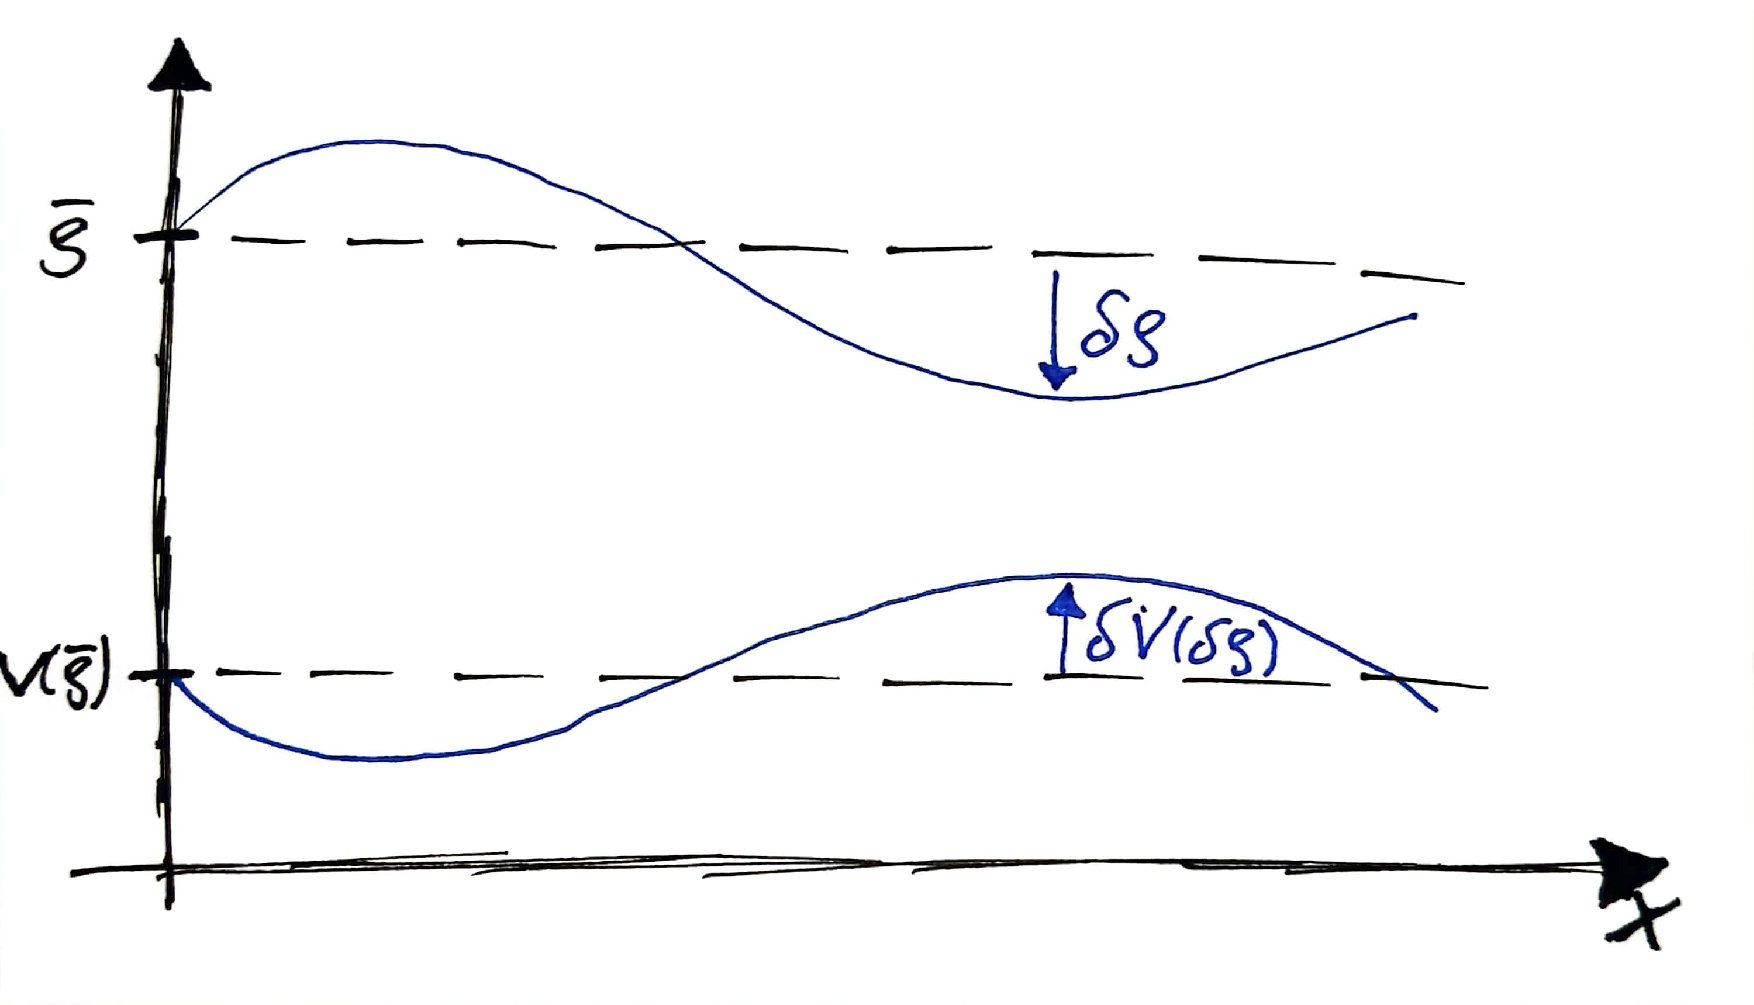
\includegraphics[width=.35\textwidth]{chapters/Figures/scalar/perturb.pdf}
    \caption{Perturbation in density gives perturbation in velocity}
    \label{fig: perturb}
\end{figure}

We now consider what happens if we pertrub a homogenous state, $\rho= \bar \rho + \delta \rho$.
Then, the velocity changes as $v(\rho) = v(\bar \rho) + \delta \rho v'(\bar \rho)$.
This will again perturb the density further, $\delta \rho'$.
Inserting this into the steady state, with $\calP = \rho$, we get
%
\begin{align}
    \bar \rho + \delta \rho'
    \propto 
    \frac{1}{v(\bar \rho) + \delta \rho v'(\bar \rho)}
    \sim \frac{1}{v(\bar \rho)} \left( 1 - \frac{\delta \rho v'(\bar \rho)}{v(\bar \rho)} \right)
    =
    \rho\left( 1 - \frac{\delta \rho v'(\bar \rho)}{v(\bar \rho)} \right)
    .
\end{align}
%
This gives a criterion for whether the perturbations are growing in strength or diminishing in strength.
If $\delta \rho' > \delta \rho$, the system is unstable.
This happens if
%
\begin{align}
    \frac{\bar \rho v'(\bar \rho)}{v(\rho)} < -1.
\end{align}
%




\subsection{Moment expansion}

To find the full dynamics of the particle density
%
\begin{align} \label{scalar order parameter}
    \rho(\bm x, t) = \int\limits _0^{2\pi} \dd \phi\, \calP(\bm x, \phi, t),
\end{align}
%
we must apply the \emph{moment expansion}.
We will see that the dynamics of $\rho$, which is the first moment of the probability distribution $\calP(\phi)$, will depend on the higher moments of the distribution.
This creates a hierarchy of equations, which we will argue can be truncated, yielding a closed set of equations.
In addition to the particle density~\autoref{scalar order parameter}, also called the scalar order parameter, the relevant moments are the polar and nematic order fields,
%
\begin{align}
    \label{polar order parameter}
    \rho(\bm x, t) p_i(\bm x, t)
    & =
    \int\limits_0^{2\pi} \dd \phi \, \hat {e}_i(\phi) \calP(\bm x, \phi, t),
    \\\label{nematic order parameter}
    \rho(\bm x, t) Q_{ij}(\bm x, t)
    & = \int\limits_0^{2 \pi} \dd \phi
    \left[
        \hat e_i(\phi)\hat e_j(\phi) - \frac{1}{2} \delta_{ij}
    \right] \calP(\bm r, \phi, t).
\end{align}
%
The polar order parameter, $p_i$, measures how much the particles align in the same direction.
If the distribution of particles is independent of the direction $\phi$, then using the explicit form of $\hat {\bm e}$, \autoref{unit vector}, we see that the polar order parameter vanishes: $\bm p = \frac{1}{2\pi} \int_0^{2\pi}\hat {\bm e}(\phi) = \bm 0$.
If the distribution is strongly peaked around some angle $\theta$, so we can approximate $\calP(\bm x, \phi, t) \propto \delta(\phi - \theta)$, then $\bm p = \hat{\bm e}(\theta)$.
In general, the polar order parameter will take on values between these extremes, varying as a function of space and time.

While the polar order parameter $\bm p$ measures the alignment of small arrows, we can consider the nematic order parameter $Q$ measures the alignment of objects that are symmetric back to front, such as an ellipse.
If the system is completely disordered, then $Q = 0$.
If 50\% of the particles points in direction $\theta = 0$, while the rest points in the opposite direction $\theta = \pi$, the $p_i = 0$, while $Q\neq 0$.
In fact, 
%
\begin{equation}
    Q = 
    \begin{pmatrix}
        1 & 0 \\ 0 & -1
    \end{pmatrix}.
\end{equation}
%
We see that $\mathrm{Tr} Q = 0$.
This is in general true for $Q$, and is due to the Krönkecker delta in its definition.
General, higher-order moments describe the alignment of objects invariant under shorter and shorter rotations.
The polar order parameter is invariant under a $2 \pi$ rotation, the nematic under a $\pi$ rotation, and so on.\footnote{
    In quantum mechanics, we must also include fields that pick up a minus sign under rotations by $2 \pi / n$.
    These are fermionic fields, while the fields introduced here are boson fields.
}
The difference between polar and nematic ordering is shown in \autoref{fig: polar and nematic}

{\it Exercise: Explain why the matrix $\bm Q$ is defined as traceless (${\sum}_i Q_{ii} = 0$). Hint: Try to calculate its expression assuming a uniform distribution of orientations.}


\begin{figure}[!htb]
    \centering
    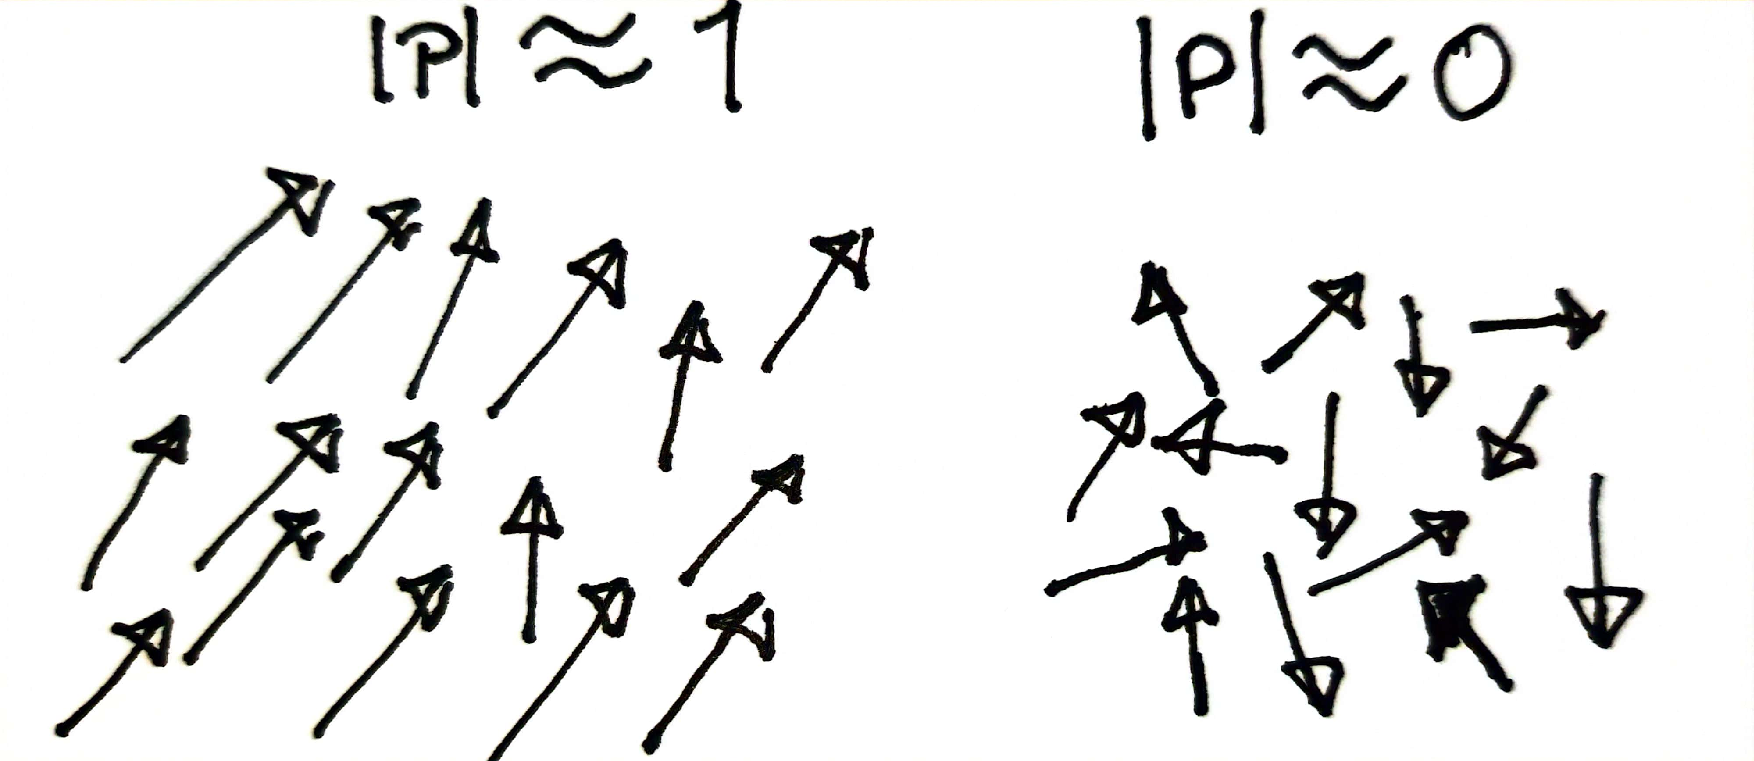
\includegraphics[width=.38\textwidth]{chapters/Figures/scalar/polar.pdf}
    \hspace{1cm}
    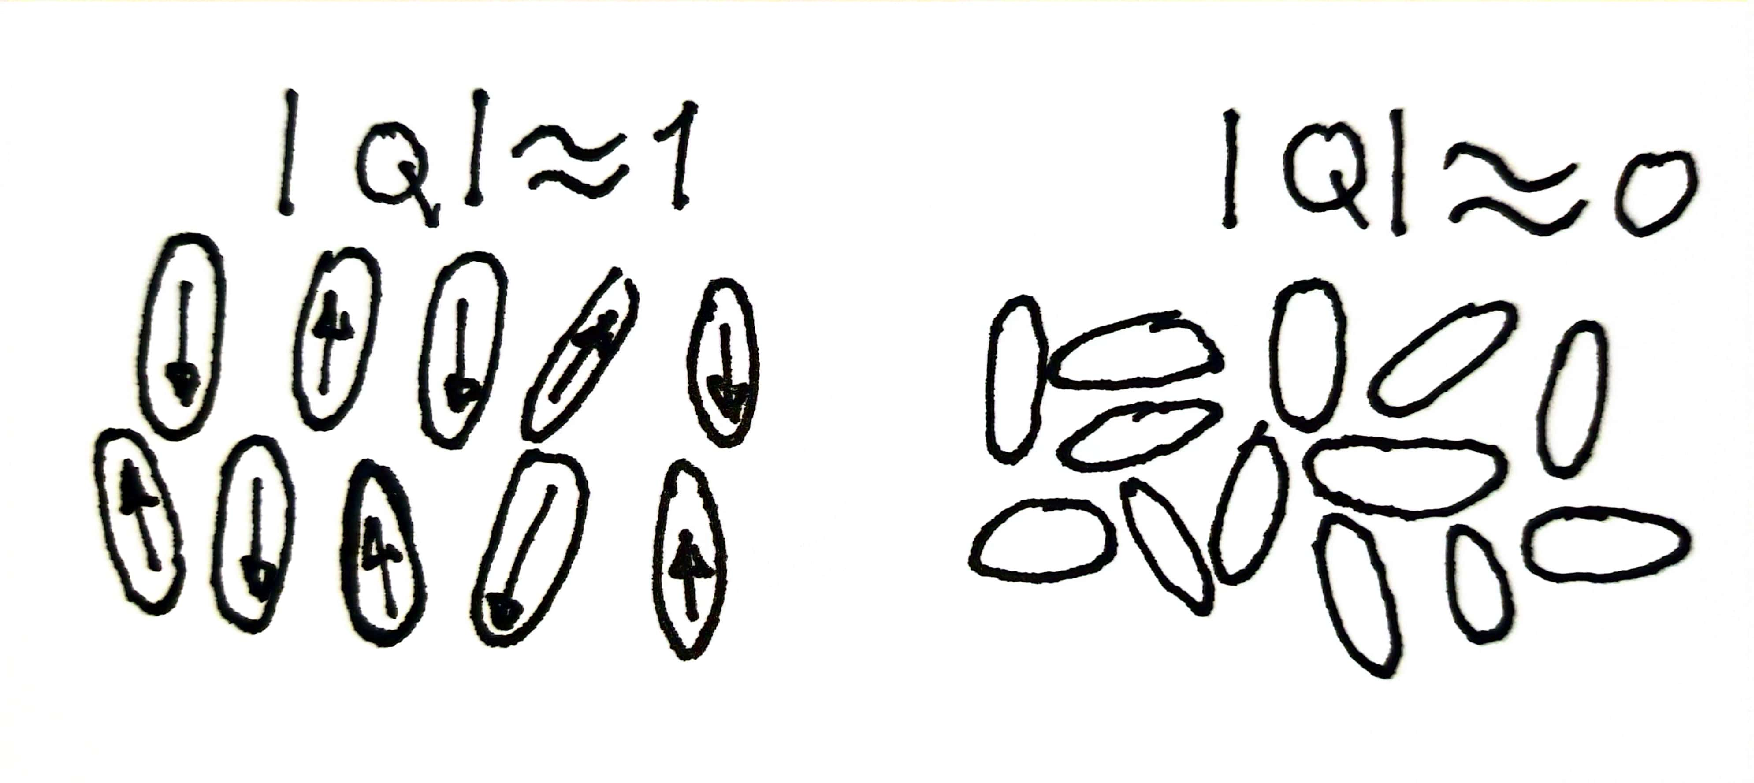
\includegraphics[width=.4\textwidth]{chapters/Figures/scalar/nematic.pdf}
    \caption{
        To the left, to configurations that have high and low polar ordering.
    To the right, two configurations which both have low polar ordering, but one has high nematic ordering, while the other has low.}
    \label{fig: polar and nematic}
\end{figure}

To derive the equations of motion of the scalar order parameter, we integrating the Fokker-Planck for the one-particle distribution over $\phi$.
In other words, we apply $\int \dd \phi$ to \autoref{eq: space dependent fokker planck}, which gives
%
\begin{align}\label{eq: density FP}
    \partial_t \rho(\bm x, t)
    = 
    - \bm \nabla \cdot [ v(\bm x, t) \rho(\bm x, t) \bm p(\bm x, t) - D \nabla \rho(\bm x, t)].
\end{align}
%
The radial diffusion term $\propto D_r$ vanishes as it is a total derivative.
% Handwritten page XI
In the same manner, we find the equation of motion for $\bm p$ by applying $\int \dd\phi \, \hat{\bm e}(\phi)$ to \autoref{eq: space dependent fokker planck}, which yields\todo[noinline]{check indices}
%
\begin{align} \label{eq: polarity FP}
    \partial_t [\rho(\bm x, t)  p_i(\bm x, t)]
    =
    -
    \nabla_{j}
    \left\{
        v(\bm x, t) \rho(\bm x, t) \left[ Q_{ij}(\bm x, t) + \frac{ 1 }{ 2 }  \delta_{ij}\right]
        - D \nabla_j [\rho p_i(\bm x, t)]
    \right\}
    - D_r \rho p_i(\bm x, t).
\end{align}
%
The last term is obtained by integration by parts.
In this equation, we are using the Einstein summation convention, which means that repeated indices are summed over.

As we can see, this expansion is a runaway process, and we need a criterion for closing this hierarchy of equations.
When we do coarse-graining, we are interested in the large-scale, long-term behavior of the system.
We therefore remove terms that are fourth order or more in gradients.
For example, the lowest order contribution to $\partial_t \rho $ is the diffusion term, so $\rho = \Oh(\nabla^2)$.
If we were to write out the equation for the nematic tensor, we would see that $Q = \Oh(\nabla)$, so $\nabla [v \rho Q] = \Oh(\nabla^4)$ and is therefore neglected.
This closes the hierarchy of equations, and we are left with
%
\begin{subequations}
\begin{align}
    \label{eq: closed density}
    \partial_t \rho(\bm x, t) &= - \nabla_i [v(\bm x, t) p_i(\bm x, t) \rho(\bm x, t) - D \nabla_i \rho(\bm x, t)], \\
    \label{eq: closed polarity}
    \partial_t [\rho(\bm x, t) p_i(\bm x, t)]
    & = 
    - \nabla_j \left[\frac{1}{2} v(\bm x, t) \rho(\bm x, t) \delta_{ij} - D\nabla_j [\rho(\bm x, t) p_i(\bm x, t)]\right] - D_r \rho(\bm x, t) p_i(\bm x, t).
\end{align}
\end{subequations}
%
As all terms in the density equation are proportional to at least one gradient term, the only time scale in this equation in this equation is the system size, $\partial_t^{-1} \sim \nabla^{-1} \sim L$, which diverges in the thermodynamic limit $L\rightarrow\infty$.
We therefore expect this dynamics to be slow.
The equation for the polar order parameter $p_i$, on the other hand, has a time scale inherited from the rotational diffusion, $\tau_r = 1 / D_r$.
In this case, we expect any non-zero polar order to relax on a time-scale $\tau_r$, which given a large enough system will be much smaller than the time scale for the density field, leading to a \emph{separation of time scales}.
\todo[inline]{This can probably be written better\dots}

To see this, consider an equation of the form
%
\begin{align} \label{eq: enslave}
    \partial_t \rho \bm p = - D_r \rho \bm p + A(\bm r, t),
\end{align}
%
we may solve it exactly as
%
\begin{align}
    \rho(\bm x, t) \bm p(\bm x,t)
    = e^{- t D_r} \left[ \rho(\bm x, 0) \bm p(\bm x,0) + \int_0^t \dd t' \, e^{- t D_r} A(\bm x,t') \right].
\end{align}
%
We will assume now that $t\gg \tau_R$, so that the first term is suppressed, and change variables to $\tau = t - t'$, which yields
%
\begin{align}
    \rho(\bm r, t) \bm p(\bm x, t)
    & = \int_0^t \dd \tau \, e^{- \tau  D_r} A(\bm x,t - \tau)\\
    & \approx
    \int_0^\infty \dd \tau \, e^{- \tau  D_r} [A(\bm x,t ) + \tau \partial_\tau A(\bm x, t) + ...]
    \approx \frac{1}{D_r} A(\bm x, t),
\end{align}
%
where we in the last step we assume $A$ does not vary much over the time-scale $\tau_R = 1 / D_R$.
This shows that, given our assumptions, we may neglect the time-derivative term in the original equation \autoref{eq: enslave}, and dynamics of $\bm p$ is now complete determined by $A(\bm x, t)$.
We say $\bm p$ is \emph{enslaved} to the slow dynamics of $A$.
Finally, we see that the diffusion term, proportional to $D$ in \autoref{eq: closed polarity}, is fourth order in gradients, and should therefore be neglected.\todo[noinline]{Is this counting right?}

We now return to the special case of a density-dependent self-propulsion velocity, $v(\bm x, t) = v(\rho(\bm x, t))$.
We can now explicitly solve for the polar order,
%
\begin{align}
    \rho p_i = 
    - \frac{1}{2 D_r} \nabla_i  [v(\rho) \rho].
\end{align}
%

A sanity check is to now substitute back in the special case $v(\rho) = v_0$, corresponding to non-interacting ABPs.
The polar order-parameter is then given by
%
\begin{align}
    \rho \bm p = - \frac{v_0}{2 D_R} \bm \nabla \rho,
\end{align}
%
which when substituted back into Fokker-Planck for the density, \autoref{eq: density FP}, gives
%
\begin{align}
    \partial_t \rho &= D_{\mathrm{eff}} \nabla^2 \rho, &
    D_{\mathrm{eff}} = D + \frac{v_0^2}{2 D_R},
\end{align}
%
which is excatly what we found in \autoref{chapter: introduction}.

% Handwritten XII

\textit{{\bf Homework}:
In two dimensions, the vector $\he(\theta) = (\cos\theta, \sin\theta)$ is parametrized by the angle $\theta_t$. Assuming that $\theta_t$ is a Markov process, justify why we can write the joint distribution as $P(\theta_2,t_2;\theta_1,t_1) = P(\theta_2-\theta_1,t_2-t_1|0,0)P(\theta_1,t_1)$ for $t_2 > t_1$.
Deduce that
\begin{equation*}
    \langle \he(\theta_t) \cdot \he(\theta_{t+\tau}) \rangle = \int \rmd\phi \cos\phi \, P(\phi,\tau|0,0) \equiv \langle \cos\phi \rangle_0, 
\end{equation*}
where $P(\theta,t)$ is the distribution of $\theta$ satisfying $P(\theta,0) = \delta(\theta)$.
(Hint: Use the properties of $\theta$ to express the joint distribution $P(\theta_2,t_2;\theta_1,t_1)$)
}



\subsection{MIPS}

If we take the more general case, where the active velocity depends on the density, $v = v(\rho)$, we may write \autoref{eq: closed density} as conservatoin law
%
\begin{align}
    \partial_t \rho(\bm x, t)  = - \bm \nabla \cdot \bm J(\bm x, t),
\end{align}
%
where the current has the form \todo[noinline]{Is the factor $\rho$ right?}
% 
\begin{align}
    J[\rho] = - \rho M[\rho] \bm \mu[\rho].
\end{align}
%
Here, we have introduced the mobility $M$ and the chemical potential $\mu$,
%
\begin{align}
    M[\rho] & = \frac{v[\rho]^2}{2 D_r},&
    \mu[\rho] & = \ln(\rho v[\rho]).
\end{align}
%
This chemical may be written as the derivative of a free energy,
%
\begin{align}
    \mu(\rho) = f'(\rho) \implies
    f(\rho) = \int^\rho \dd x \, \ln (v[x] x).
\end{align}
%
This means that we can apply the methods of equilibrium theory of phase separation.
This is detailed in \autoref{chapter: phase sep}.
If we assume there is a homogenous solution $\rho = \bar \rho$, this will be unstable if $f''(\bar \rho) < 0$.
Inserting this into the free energy we found, we get the criterion
%
\begin{align}
    \frac{v'(\bar \rho)\bar \rho}{v(\bar \rho)} < - 1.
\end{align}
%
This gives the \emph{spinodals}, where the system is unstable for any perturbation.
However, as described in \autoref{chapter: phase sep}, the new phases are described by the \emph{binodals}.
Following the procedure laid out there, we write the equations for chemical and mechanical equilibrium for the two phases with density $\bar \rho_i$ and volume $\V_i$,
%
\begin{align}
    \V_i[f'(\bar \rho_i) - \mu] &= 0, \\
    f(\bar \rho_i) - \mu \rho_i + P &= 0,
\end{align}
%
whose solution gives the volumes and density of each phase given an overall density $\bar \rho$.

This is called motility-induced phase-separation, as the mechanism of phase is not attraction, as in passive systems, but a lowering of the motility in high densities.
The mechanics of phase separation are thus non-equilibrium, however, the resulting large-scale dynamics are still described by an effective equilibrium theory.
This comes as we can always find free energy, no matter the shape of $v(\rho)$.
To break equilibrium also at the large scale, we must have a more general current.
One way to obtain this is to extend the momentum expansion to higher orders.


\section{Top-down approach: Active model B}

Another way to achieve a model with out-of-equilibrium effects is to take the Ginzbur-Landau approach and write down all possible terms allowed by symmetry and conservation.
We begin with the conservation law,
%
\begin{align}
    \partial_t \rho = - \bm \nabla \cdot \bm J,
\end{align}
%
and write the current as
%
\begin{align}
    \bm J = 
    - \rho M(\rho) \bm \nabla 
    \left[
        f'(\rho) - K \nabla^2 \rho + \lambda |\nabla \rho|^2
    \right]
    + \zeta \nabla^2 \rho \bm \nabla \rho.
\end{align}
%
The two first terms may be written in terms of a free energy functional.
The two next cannot, due to the gradient structure.
With only the $\lambda$ term, this is called the active model B.
It was later discovered that another term was possible to include, namely the $\zeta$ term.
With this addition, the model is called active model B+.
More details on this model are given in \autoref{section: active model B top down}.





